\documentclass{article}
% translate with >> pdflatex -shell-escape <file>

% This file is used as unit test for pgfplots, copyright by Christian Feuersaenger.
% 
% See
%   http://pgfplots.sourceforge.net/pgfplots.pdf
% for pgfplots.
%
% Any required input files (for <plot table> or <plot file> or the table package) can be downloaded
% at
% http://www.ctan.org/tex-archive/graphics/pgf/contrib/pgfplots/doc/latex/
% and
% http://www.ctan.org/tex-archive/graphics/pgf/contrib/pgfplots/doc/latex/plotdata/

\usepackage{pgfplots}
\pgfplotsset{compat=1.3}

\pagestyle{empty}

\begin{document}
	\pgfplotsset{
		xtick={-1,-0.5,...,1.001},
	}
		
	Here, a $-0.5$ penetrated the axis in an earlier version, should be fixed now:
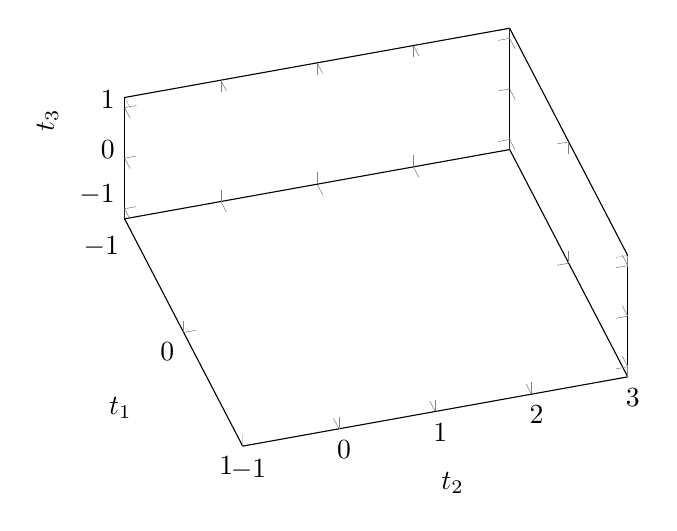
\begin{tikzpicture}
		\begin{axis}[clip=false,
			xmin=-1,xmax=1,
			ymin=-1,ymax=3,
			zmin=-1,zmax=1,
			enlarge z limits,
			xlabel=$t_1$,ylabel=$t_2$,zlabel=$t_3$,width=8cm,view/h=73,view/v=63]

		\end{axis}
	\end{tikzpicture}
\end{document}
